\apendice{Especificación de permisos}

\section{Roles Predefinidos en PAM360}

PAM360 proporciona varios roles predefinidos, cada uno con un conjunto específico de permisos que determinan las acciones que los usuarios pueden o no pueden realizar dentro del sistema. Estos roles están diseñados para cubrir las necesidades seguridad de la plataforma y es uno de los principales sentidos de su uso. A continuación, se describen los roles y sus permisos:

\subsection{Privileged Administrator (Administrador Privilegiado)}
\begin{itemize}
	\item \textbf{Descripción}: Este rol tiene privilegios similares a los de un administrador predeterminado, pero con capacidades adicionales para configurar la privacidad y los controles de seguridad.
	\item \textbf{Permisos}:
	\begin{itemize}
		\item Manage Users (Gestionar Usuarios)
		\item Manage Resources (Gestionar Recursos)
		\item Manage Passwords (Gestionar Contraseñas)
		\item View Passwords (Ver Contraseñas)
		\item Managing Personal Passwords (Gestionar Contraseñas Personales)
		\item View Audit and Reports (Ver Auditorías y Reportes)
		\item Privacy and Security Controls (Controles de Privacidad y Seguridad)
		\item Remote Access, File Transfer, and Remote App Access (Acceso Remoto, Transferencia de Archivos y Acceso a Aplicaciones Remotas)
	\end{itemize}
\end{itemize}

\subsection{Administrator (Administrador)}
\begin{itemize}
	\item \textbf{Descripción}: Este rol permite la creación, configuración y administración de recursos y usuarios, así como la gestión de contraseñas y la visualización de auditorías y reportes.
	\item \textbf{Permisos}:
	\begin{itemize}
		\item Manage Users
		\item Manage Resources
		\item Manage Passwords
		\item View Passwords
		\item Managing Personal Passwords
		\item View Audit and Reports
	\end{itemize}
\end{itemize}

\subsection{Password Administrator (Administrador de Contraseñas)}
\begin{itemize}
	\item \textbf{Descripción}: El administrador de contraseñas tiene la capacidad de gestionar y visualizar todas las contraseñas en el sistema, excepto las contraseñas personales de otros usuarios.
	\item \textbf{Permisos}:
	\begin{itemize}
		\item Manage Passwords
		\item View Passwords
		\item Managing Personal Passwords
	\end{itemize}
\end{itemize}

\subsection{Password Auditor (Auditor de Contraseñas)}
\begin{itemize}
	\item \textbf{Descripción}: Este rol está enfocado en la auditoría y revisión de las contraseñas sin la capacidad de realizar cambios.
	\item \textbf{Permisos}:
	\begin{itemize}
		\item View Passwords
		\item View Audit and Reports
	\end{itemize}
\end{itemize}

\subsection{Password User (Usuario de Contraseñas)}
\begin{itemize}
	\item \textbf{Descripción}: Los usuarios con este rol pueden ver las contraseñas que se han compartido con ellos por los administradores.
	\item \textbf{Permisos}:
	\begin{itemize}
		\item View Passwords
		\item Managing Personal Passwords
	\end{itemize}
\end{itemize}

\subsection{Connection User (Usuario de Conexión)}
\begin{itemize}
	\item \textbf{Descripción}: Este rol permite a los usuarios tomar conexiones remotas y realizar transferencias de archivos.
	\item \textbf{Permisos}:
	\begin{itemize}
		\item Remote Access, File Transfer, and Remote App Access
	\end{itemize}
\end{itemize}

\subsection{Resumen de Permisos por Rol}

\begin{figure}[H]
	\centering
	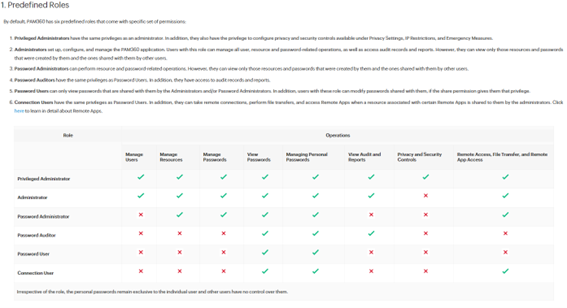
\includegraphics[width=0.8\textwidth]{./img/pam_roles.png}
	\caption{roles PAM360.}
	\label{fig:pam_rol}
\end{figure}


